\section{Steady state spectroscopy}
\label{sec:SSS}

\subsection{Structural influences}

In the following, the steady state spectra for ZnTPP and ZnOEP in the two solvents toluene (Tol) and benzonitrile (BN) are analyzed.

First, we are comparing the spectra of the two different materials ZnTPP and ZnOEP as depicted in \cref{fig:ZnTPPZnOEP}. The measured data is in great accordance with 
literature \cite{Wagner.1994}.
\begin{figure}[h]
    \centering
    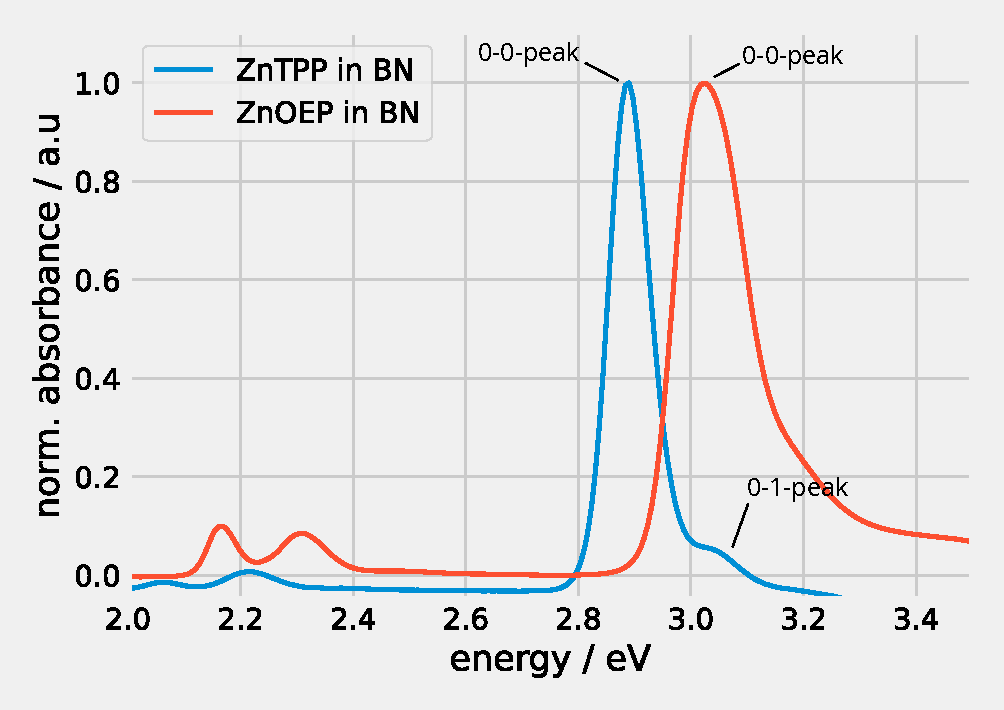
\includegraphics[width = 12cm]{Program/ZnTPPZnOEP.pdf}
    \caption{UV / VIS spectrum of ZnTPP and ZnOEP in benzonitrile.}
    \label{fig:ZnTPPZnOEP}
\end{figure}
The peak positions are analyzed using \textit{scipy.optimize.curve\_fit()}. The absorption spectrum consists of four bands in our detected range. The Soret band $S_\mathrm{2}$ (B-band) of ZnTPP peaks at 
\SI{2.89 \pm 0.01}{\eV}, while the weaker band at \SI{3.05\pm0.03}{\eV} can be assigned to a convolution of transitions of vibrational bands \cite{Even.1982}.
The two bands in the in the range of of 2 to \SI{2.4}{\eV} are the Q-bands. 

For ZnOEP the Sorbet peak occurs at \SI{3.03\pm 0.02}{\eV}. This gives clear blue shift compared to ZnTPP.
This shift in the peak position can be explained by investigating the structure of the the two molecules. As shown in (ref), ZnTPP differs structurally from ZnOEP by having four benzene rings.
These enlarge the system of conjugated $\pi$-bonds, which leads to a lowering of the absorption energy\cite{Kohler.2015}. Intuitively, we can
understand this by imagining the system of conjugated bonds as a box as often treated in quantum mechanics.
Therefore it seem plausible that enlarging the box lowers the energy levels.

\subsection{Influence of solvent}

The fact that the choice of solvent during UV / VIS spectroscopy changes the position of the absorption \cite{Parson.2015}. There are multiple effects, changing the positions such as reorganisation of 
the solvent around the molecule when the molecule performs a transitions from the ground state to the exited state as the symmetry and charge distribution changes. Furthermore, the conformation
of the molecule can change with the choice of solvents. A easily understandable example would be the a unpolar chain of carbon atoms. In a polar solvent, this chain would form a coil as it would have less interaction with 
the solvent whereas in a unpolar solvent it might stretch out and show a more planare backbone. 
In our case we see a difference in the peak position 